% !TEX TS-program = pdflatex
%%%%%%%%%%%%%%%%%%%%%%%%%%%%%%%%%%%%%%%%%%%%%%%%%%%%%%%%%%%%%%%
%
%     filename  = "YourName-Dissertation.tex",
%     version   = "1.6.0",
%     date      = "2018/03/25",
%     authors   = "Gary L. Gray,
%     copyright = "Gary L. Gray",
%     address   = "Engineering Science and Mechanics,
%                  212 Earth & Engineering Sciences Bldg.,
%                  Penn State University,
%                  University Park, PA 16802,
%                  USA",
%     telephone = "814-863-1778",
%     email     = "gray@psu.edu",
%
%%%%%%%%%%%%%%%%%%%%%%%%%%%%%%%%%%%%%%%%%%%%%%%%%%%%%%%%%%%%%%%
%
% Change History:
%
% 1.6.0	**	Substantial changes to the title page and signature
%			that are generated for bachelors theses.
%
%		**	honorsdepthead has been changed to escdepthead since
%			Engineering Science is the only department at Penn
%			that requires the department head's signature. Ugh.
%
%		**	honorsdegreeinfo has been changed to bachelorsdegreeinfo
%			to reflect the fact that all Engineering Science
%			students write a thesis, but not all graduate with
%			honors.
%
%		**	Removed the honors class option.
%
%		**	Added the esc class option for Engineering Science
%			students. This puts the department head's name on the
%			title page and adds their sig to the signature page.
%
%		**	Added the schreyer option properly format the title page
%			and signature page for students in the Schreyer Honors
%			College.
%
%		**	Added deptheadtitle command for Engineering Science
%			students.
%
%		**	Added the twoha option for students with interdisciplinary
%			honors and thus with two honors advisors.
%
%		**	Updated and revised some of the instructions below based on %			the above changes.
%
% 1.4.0	**	Added two documents in a "LaTeX Help" folder. They should
%			be helpful for people who are new to LaTeX.
%
%		**	Added some equations, figures, a table to Chapter 1 to
%			provide some examples.
%
% 1.3.0	**	Added the cite package.
%
%		**	Give that the Graduate School now allows essentially
%			any line spacing, I have moved the line space setting
%			from psuthesis.cls to this driver file. Go ahead and
%			make it ugly if you want. :-)
%
%		**	Removed \addtocounter{page}{-1} after \psutitlepage is
%			executed. It made the paging of the frontmatter
%			incorrect. I can no longer remember why it was there.
%
%		**	Removed \psusigpage since the Graduate School now
%			provides the signature page.
%
%		**	Added the command \collegesubmittedto to add the College
%			in which the thesis/dissertation has been completed to
%			the title page.
%
%		**	Added instructions for documents that include a single
%			appendix since the Graduate School just hates calling it
%			``Appendix A'' if there is a single appendix.
%
%		**	Removed the fncychap package since I could not easily
%			find a way to make it work with documents that have a
%			single appendix.
%
%		**	Added the titlesec package so that the user can make the
%			format of the chapter titles a little less boring than
%			LaTeX's default.
%
% 1.2.2	**	Added some information to the main driver file (this
%			file) regarding the use of hyperref with the
%			psuthesis class. Thanks to Nathan Urban for pointing
%			out the included workaround.
%
% 1.2.1	**	Finally reproduced and fixed the problem where the
%			page number listed in the TOC for the Bibliography
%			was the last page number of the Bibliography.
%
%		**	Added 10pt and 11pt options to the document class,
%			though I have no idea why anyone would want to use
%			such insanely small font sizes since it will lead to
%			line lengths that are much too long.
%
% 1.2.0	**	Two additional class options have been added to
%			support honors theses submitted to the Schreyer
%			Honors College. These options are:
%			- honors
%			- honorsdepthead
%			See below for details.
%
%		**	I have also added the commands:
%			- honorsdegreeinfo
%			- honorsadvisor
%			- honorsdepthead
%			Again, see below for details.
%
% 1.1.2	**	If you want to use the subfigure package with our
%			psuthesis class file, then you must must find the 
%			following line in the psuthesis.cls file:
%
%			\RequirePackage{tocloft}
%
%			and add the subfigure option. I have already set
%			this up for you in the psuthesis.cls file to make
%			this easy to do.
%
% 1.1.1	**	Added the fncychap package to the distribution.
%
% 1.1.0	**	The way that the thesis frontmatter and backmatter
%			is generated has been completely re-done in order
%			to be more intuitive.
%
%		**	I have added the ability to change the title of
%			the Dedication/Epigraph to anything you please.
%
%		**	In the process of changing the format of the Table
%			of Contents to conform to the inflexible rules of
%			the Grad School (the word ``Chapter'' and
%			``Appendix'' need to appear before the number and
%			letter, respectively), I have added an option to
%			the class called inlinechaptertoc that changes the
%			format of the Chapter/Appendix entries in the TOC.
%			Note that the tocloft package is now required.
%
%		**	Appendices should now start with the
%			\Appendix command rather than \chapter. See the
%			accompanying files for examples.
%
%		**	Added information regarding the Nontechnical
%			Abstract that is required of ESM students.
%
%		**	Added the fncychap package for those of you who like
%			the nice Chapter headings it provides. I like
%			Lenny, but you don't have to use it if you don't
%			want to. In addition, the other options are: Sonny,
%			Glenn, Conny, Rejne, and Bjarne
%
% 1.0.4	**	fixed the \addcontentsline entry for BibTeX within
%			the commented out text in the Bibliography section
%
% 1.0.3	**	added a sigpage option to conform to new Grad School
%			requirements
%
% 1.0.2	**	issued the \appendix command to start the appendices
%
%		**	moved the \addcontentsline for the bibliography so
%			that the bibliography now shows up on the right page
%			in the TOC
%
%		**	added some info if you use bibtex
%
% 1.0.1	**	eqlist and eqparbox are now included in the archive
%
%%%%%%%%%%%%%%%%%%%%%%%%%%%%%%%%%%%%%%%%%%%%%%%%%%%%%%%%%%%%%%%
%
% This is a template file to help get you started using the
% psuthesis.cls for theses and dissertations at Penn State
% University. You will, of course, need to put the
% psuthesis.cls file someplace that LaTeX will find it.
%
% I have set up a directory structure that I find to be clean
% and convenient. You can readjust it to suit your tastes. In
% fact, the structure used by our students is even a little
% more involved and commands are defined to point to the
% various directories.
%
% This document has been set up to be typeset using pdflatex.
% About the only thing you will need to change if typesetting
% using latex is the \DeclareGraphicsExtensions command.
%
% The psuthesis document class uses the same options as the
% book class. In addition, it requires that you have the
% ifthen, calc, setspace, and tocloft packages.
%
% The first additional option specifies the degree type. You
% can choose from:
%	Ph.D. using class option <phd>
%	M.S. using class option <ms>
%	M.Eng. using class option <meng>
%	M.A. using class option <ma>
%	B.S. using class option <bs>
%	B.A. using class option <ba>
%	Honors from the Schreyer Honors College <schreyer>
%
% The second additional option inlinechaptertoc determines
% the formatting of the Chapter entries in the Table of
% Contents. The default sets them as two-line entries (try it).
% If you want them as one-line entries, issue the
% inlinechaptertoc option.
%
% The class option schreyer should be used for theses
% submitted to the Schreyer Honors College.
%
% The class option esc should be used by all Engineering Science
% students.
%
% The option option twoha should be used if you are earning
% interdisciplanary honors and thus have two honors advisors.
%
% The class option ``secondthesissupervisor'' should be used
% for baccalaureate honors degrees if you have a second
% Thesis Supervisor.
%
% The vita is only included with the phd option and it is
% placed at the end of the thesis. The permissions page is only
% included with the ms, meng, and ma options.
%%%%%%%%%%%%%%%%%%%%%%%%%%%%%%%%%%%%%%%%%%%%%%%%%%%%%%%%%%%%%%%
% Only one of the following lines should be used at a time.
% Doctoral students.
%\documentclass[phd,12pt]{psuthesis}
% Masters students
%\documentclass[ms,12pt]{psuthesis}
% Bachelors students in the Schreyer Honors College.
%\documentclass[bs,schreyer,12pt]{psuthesis}
% Bachelors students in the Schreyer Honors College & Engineering Science.
%\documentclass[bs,schreyer,esc,twoha,12pt]{psuthesis}
% Bachelors students in Engineering Science.
\documentclass[bs,schreyer,12pt]{psuthesis}

\usepackage[T1]{fontenc}
%\usepackage{lmodern}
\usepackage{textcomp}
\usepackage{microtype}

%%%%%%%%%%%%%%%%%%%%%%%%%%%
% Packages I like to use. %
%%%%%%%%%%%%%%%%%%%%%%%%%%%
\usepackage{amsmath}
\usepackage{amssymb}
%\usepackage{amsthm}
%\usepackage{exscale}
%\usepackage[mathscr]{eucal}
%\usepackage{bm}
\usepackage{xspace}
\usepackage{subfigure}
\usepackage{eqlist} % Makes for a nice list of symbols.
\usepackage[nosepfour,warning,np,debug,autolanguage]{numprint}
\usepackage{acro}
\usepackage{booktabs}
\usepackage[final]{graphicx}
\usepackage[dvipsnames]{color}
\DeclareGraphicsExtensions{.pdf, .jpg}

\usepackage{url}

% http://www.tex.ac.uk/cgi-bin/texfaq2html?label=citesort
\usepackage[sorting,compression]{cite}

\usepackage{titlesec}

%%%%%%%%%%%%%%%%%%%%%%%%%%%%%%%
% Use of the hyperref package %
%%%%%%%%%%%%%%%%%%%%%%%%%%%%%%%
%
% This is optional and is included only for those students
% who want to use it.
%
% To the hyperref package, uncomment the following line:
%\usepackage{hyperref}
%
% Note that you should also uncomment the following line:
%\renewcommand{\theHchapter}{\thepart.\thechapter}
%
% to work around some a problem hyperref has with the fact
% the psuthesis class has unnumbered pages after which page
% counters are reset.

% Set the baselinestretch using the setspace package.
% The LaTeX Companion claims that a \baselinestretch of
% 1.24 gives one-and-a-half line spacing, which is allowed
% by the PSU thesis office. As of October 18, 2013, the Graduate
% School states ``The text of an eTD may be single-, double- or
% one- and-a-half-spaced.'' Go nuts!
\setstretch{1.24}


%%%%%%%%%%%%%%%%%%%%%%%%%%%%%%%%%%%%
% SPECIAL SYMBOLS AND NEW COMMANDS %
%%%%%%%%%%%%%%%%%%%%%%%%%%%%%%%%%%%%
% Place user-defined commands below.

% Define the \acro command.
\makeatletter
\newif\ifFirstPar       \FirstParfalse
\def\smc{\sc}
\def\ninepoint{\small}
\DeclareRobustCommand\SMC{%
  \ifx\@currsize\normalsize\small\else
   \ifx\@currsize\small\footnotesize\else
    \ifx\@currsize\footnotesize\scriptsize\else
     \ifx\@currsize\large\normalsize\else
      \ifx\@currsize\Large\large\else
       \ifx\@currsize\LARGE\Large\else
        \ifx\@currsize\scriptsize\tiny\else
         \ifx\@currsize\tiny\tiny\else
          \ifx\@currsize\huge\LARGE\else
           \ifx\@currsize\Huge\huge\else
            \small\SMC@unknown@warning
 \fi\fi\fi\fi\fi\fi\fi\fi\fi\fi
}
\newcommand\SMC@unknown@warning{\TBWarning{\string\SMC: unrecognised
    text font size command -- using \string\small}}
\newcommand\textSMC[1]{{\SMC #1}}
\newcommand\acro[1]{\textSMC{#1}\@}

\makeatother

% command for vectors
\newcommand{\bv}[1]{\ensuremath{\vec{#1}}}
% command for unit vectors
\newcommand{\uv}[2][blank]{%
\ifthenelse{\equal{#1}{blank}}%
{\ensuremath{\hat{u}_{#2}}}%
{}%
%
\ifthenelse{\equal{#1}{.}}%
{\ensuremath{\dot{\hat{u}}_{#2}}}%
{}%
%
\ifthenelse{\equal{#1}{'}}%
{\ensuremath{\hat{u}'_{#2}}}%
{}%
}
\newcommand{\ui}{\ensuremath{\hat{\imath}}}
\newcommand{\uj}{\ensuremath{\hat{\jmath}}}
\newcommand{\uk}{\ensuremath{\hat{k}}}


%%%%%%%%%%%%%%%%%%%%%%%%%%%%%%%%%%%%%%%%%
% Renewed Float Parameters              %
% (Makes floats fit better on the page) %
%%%%%%%%%%%%%%%%%%%%%%%%%%%%%%%%%%%%%%%%%
\renewcommand{\floatpagefraction}{0.85}
\renewcommand{\topfraction}      {0.85}
\renewcommand{\bottomfraction}   {0.85}
\renewcommand{\textfraction}     {0.15}

% ----------------------------------------------------------- %

%%%%%%%%%%%%%%%%
% FRONT-MATTER %
%%%%%%%%%%%%%%%%
% Title
\title{Dynamics of Fish}

% Author and Department
\author{Michael Mazza}
\dept{Mechanical Engineering}
% the degree will be conferred on this date
\degreedate{May 2019}
% year of your copyright
\copyrightyear{2019}

% This command is used for students submitting a thesis to the
% Schreyer Honors College and for students in Engineering Science.
% The argument of this command should contain every after the word
% ``requirements'' that appears on the title page. This provides the
% needed flexibility for all the degree types.
\bachelorsdegreeinfo{for a baccalaureate degree \\ in Mechanical Engineering \\ with honors in Mechanical Engineering}

% This is the document type. For example, this could also be:
%	Comprehensive Document
%	Thesis Proposal
\documenttype{Thesis}
%\documenttype{Dissertation}
%\documenttype{Comprehensive Document}


% This will generally be The Graduate School, though you can
% put anything in here to suit your needs.
\submittedto{The Graduate School}

% This is the college to which you are submitting the
% thesis/dissertation.
\collegesubmittedto{College of Engineering}


%%%%%%%%%%%%%%%%%%
% Signatory Page %
%%%%%%%%%%%%%%%%%%
% You can have up to 7 committee members, i.e., one advisor
% and up to 6 readers.
%
% Begin by specifying the number of readers.
\numberofreaders{3}

% For baccalaureate honors degrees, enter the name of your
% honors advisor below.
\honorsadvisor{Stephanie Stockar}
{Assistant Professor of Mechanical Engineering}
%\honorsadvisortwo{Honors P. Advisor, Jr.}
%{Professor of Engineering Science and Mechanics}

% For baccalaureate honors degrees, if you have a second
% Thesis Supervisor, enter his or her name below.
\secondthesissupervisor{Second T. Supervisor}

% For baccalaureate honors degrees, certain departments
% (e.g., Engineering Science and Mechanics) require the
% signature of the department head. In that case, enter the
% name and title of your department head below.
\escdepthead{Department Q. Head}
\escdeptheadtitle{P. B. Breneman Chair and Professor 
of Engineering Science and Mechanics
}

% Input reader information below. The optional argument, which
% comes first, goes on the second line before the name.
\advisor[Thesis Advisor, Chair of Committee]
		{Francesco Costanzo}
		{Professor of Engineering Science and Mechanics}

\readerone[Optional Title Here]
			{Reader Name}
			{Professor of SomeThing}

\readertwo[Optional Title Here]
			{Reader Name}
			{Professor of SomeThing}

\readerthree[Optional Title Here]
			{Reader Name}
			{Professor of SomeThing}

\readerfour[Optional Title Here]
			{Reader Name}
			{Professor of SomeThing}

\readerfive[Optional Title Here]
			{Reader Name}
			{Professor of SomeThing}

% Format the Chapter headings using the titlesec package.
% You can format section headings and the like here too.
\definecolor{gray75}{gray}{0.75}
\newcommand{\hsp}{\hspace{15pt}}
\titleformat{\chapter}[display]{\fontsize{30}{30}\selectfont\bfseries\sffamily}{Chapter \thechapter\hsp\textcolor{gray75}{\raisebox{3pt}{|}}}{0pt}{}{}

\titleformat{\section}[block]{\Large\bfseries\sffamily}{\thesection}{12pt}{}{}
\titleformat{\subsection}[block]{\large\bfseries\sffamily}{\thesubsection}{12pt}{}{}


% Makes use of LaTeX's include facility. Add as many chapters
% and appendices as you like.
\includeonly{%
Chapter-1/Chapter-1,
Chapter-2/Chapter-2,
Chapter-3/Chapter-3,
%Chapter-4/Chapter-4,%
%Chapter-5/Chapter-5,%
%Appendix-A/Appendix-A,%
%Appendix-B/Appendix-B,%
%Appendix-C/Appendix-C,%
%Appendix-D/Appendix-D,%
%Appendix-E/Appendix-E%
}

\usepackage{listings}
%%%%%%%%%%%%%%%%%
% THE BEGINNING %
%%%%%%%%%%%%%%%%%
\begin{document}
%%%%%%%%%%%%%%%%%%%%%%%%
% Preliminary Material %
%%%%%%%%%%%%%%%%%%%%%%%%
% This command is needed to properly set up the frontmatter.
\frontmatter

%%%%%%%%%%%%%%%%%%%%%%%%%%%%%%%%%%%%%%%%%%%%%%%%%%%%%%%%%%%%%%
% IMPORTANT
%
% The following commands allow you to include all the
% frontmatter in your thesis. If you don't need one or more of
% these items, you can comment it out. Most of these items are
% actually required by the Grad School -- see the Thesis Guide
% for details regarding what is and what is not required for
% your particular degree.
%%%%%%%%%%%%%%%%%%%%%%%%%%%%%%%%%%%%%%%%%%%%%%%%%%%%%%%%%%%%%%
% !!! DO NOT CHANGE THE SEQUENCE OF THESE ITEMS !!!
%%%%%%%%%%%%%%%%%%%%%%%%%%%%%%%%%%%%%%%%%%%%%%%%%%%%%%%%%%%%%%

% Generates the title page based on info you have provided
% above.
\psutitlepage

% Generates the committee page -- this is bound with your
% thesis. If this is an baccalaureate honors thesis, then
% comment out this line.
%\psucommitteepage

% Generates the abstract. The argument should point to the
% file containing your abstract. 
\thesisabstract{SupplementaryMaterial/Abstract}

% Generates the Table of Contents
\thesistableofcontents

% Generates the List of Figures
\begin{singlespace}
\renewcommand{\listfigurename}{\sffamily\Huge List of Figures}
\setlength{\cftparskip}{\baselineskip}
\listoffigures
\end{singlespace}
\clearpage

% Generates the List of Tables
\begin{singlespace}
\renewcommand{\listtablename}{\sffamily\Huge List of Tables}
\setlength{\cftparskip}{\baselineskip}
\listoftables
\end{singlespace}
\clearpage

% Generates the List of Symbols. The argument should point to
% the file containing your List of Symbols. 
\thesislistofsymbols{SupplementaryMaterial/ListOfSymbols}

% Generates the Acknowledgments. The argument should point to
% the file containing your Acknowledgments. 
\thesisacknowledgments{SupplementaryMaterial/Acknowledgments}

% Generates the Epigraph/Dedication. The first argument should
% point to the file containing your Epigraph/Dedication and
% the second argument should be the title of this page. 
%\thesisdedication{SupplementaryMaterial/Dedication}{Dedication}



%%%%%%%%%%%%%%%%%%%%%%%%%%%%%%%%%%%%%%%%%%%%%%%%%%%%%%
% This command is needed to get the main part of the %
% document going.                                    %
%%%%%%%%%%%%%%%%%%%%%%%%%%%%%%%%%%%%%%%%%%%%%%%%%%%%%%
\thesismainmatter

%%%%%%%%%%%%%%%%%%%%%%%%%%%%%%%%%%%%%%%%%%%%%%%%%%
% This is an AMS-LaTeX command to allow breaking %
% of displayed equations across pages. Note the  %
% closing the "}" just before the bibliography.  %
%%%%%%%%%%%%%%%%%%%%%%%%%%%%%%%%%%%%%%%%%%%%%%%%%%
\allowdisplaybreaks{
%\pagestyle{fancy}
%\fancyhead{}
%
%%%%%%%%%%%%%%%%%%%%%%
% THE ACTUAL CONTENT %
%%%%%%%%%%%%%%%%%%%%%%
% Chapters
% !TEX root = ../YourName-Dissertation.tex
%
\chapter{Introduction} \label{chapter1:introduction}
%
My journey in writing this thesis started with an interest in research in the biomedical engineering field. I participated in a summer REU (Research Experience for Undergraduates) at Penn State, my initial project that I was involved with was investigating  a computational model of blood under various flow conditions. After that summer, I started down the path to write this thesis in earnest. The mathematical model that describes the flood of blood has terms that are typical of advection, reaction, and diffusion problems. Among the many mathematical features of the blood model, two particular ones present some issues when solved numerically. The focus of this thesis shifted from the actual model to the problem features of the model. The two specific features that the blood model exhibits are advection behavior in flows and the inf-sup condition. These features are not specific to the model for blood. In fact they can be demonstrated separately in simple 1D examples that will be presented later in this chapter.


Advection behavior occurs when the gradient of a field, say $\phi$, is multiplied by a velocity as in the term $\nabla\phi\cdot\bv{v}$. This behavior can be seen in the Navier-Stokes equations. In the Navier-Stokes problem the advection term is $(\nabla\bv{v})\bv{v}$. The Navier-Stokes equations also exhibit the inf-sup condition. The inf-sup condition comes from constraints that are enforced through Lagrange multipliers. The Lagrange multiplier in the Navier-Stokes equations is the incompressibility equation \textit{i.e.} $\nabla\cdot\bv{v} = 0$. The term $det\,\tensor{B_{\kappa}}=1$ in the blood model is a similar constraint that results in the inf-sup condition.
%
\section{Advection-Dominated Flow}
In order to demonstrate the numerical difficulties that advection-dominated flows present, we will consider an example with both the finite difference method and the finite element method. Consider the 1D advection-diffusion BVP,
\begin{align}
    \label{1d advec}
    u\, \partial_{x}\phi &= k\, \partial_{xx}\phi
    \\
    \label{1d advec bc1}
    \phi\,(0) &= 0
    \\
    \label{1d advec bc2}
    \phi\,(L) &= 1
\end{align}
where $u$ is the given flow velocity and $k$ is the diffusivity of $\phi$. \textcolor{red}{Please define L.} We assume that both $u$ and $k$ are positive and constant. The exact solution to the BVP stated in Eqs.~\eqref{1d advec}--\eqref{1d advec bc2} is
\begin{equation}
    \phi= \frac{1-e^{\frac{Pe\,x}{L}}}{1-e^{Pe}},
\end{equation}
where $Pe$ is the global Peclet number ($Pe=u\,L/k$). We can also define an elemental Peclet number $\alpha$ as
\begin{equation}
    \alpha=\frac{u\,h}{2k},
\end{equation}
%%
\textcolor{red}{where $h$ is ?}
\begin{figure}
    \centering
    %\begin{subfigure}
        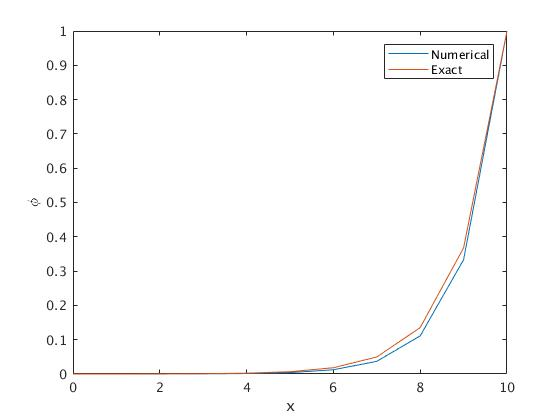
\includegraphics[width=0.3\textwidth]{../Chapter-1/Figures/alpha_5}
        \caption{$\alpha=0.5$}
      %  \label{fig:alpha=.5}
    %\end{subfigure}
    %\begin{subfigure}
       % \includegraphics[width=0.3\textwidth]{../Chapter-1/Figures/alpha}
        %\caption{$\alpha=1$}
      %  \label{fig:alpha=1}
    %\end{subfigure}
    %\begin{subfigure}
        %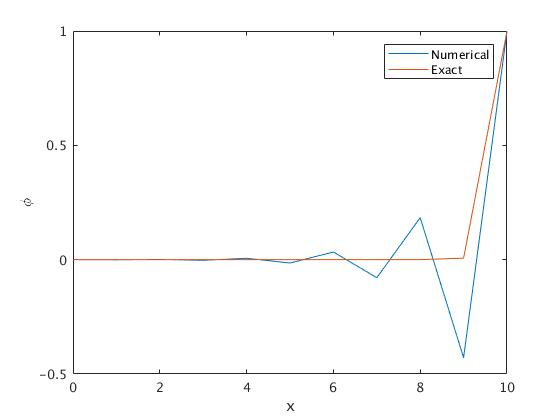
\includegraphics[width=0.3\textwidth]{../Chapter-1/Figures/alpha2_5}
        % \caption{$\alpha=2.5$}
     %   \label{fig:alpha=2.5}
    %\end{subfigure}
\end{figure}
% !TEX root = ../YourName-Dissertation.tex

\chapter{Title of the Second Chapter}

\section{Introduction}
When in the Course of human events, it becomes necessary for one people  to dissolve the political bands which have connected them with another,  and to assume among the powers of the earth, the separate and equal station  to which the Laws of Nature and of Nature's God entitle them, a decent respect to the opinions of mankind requires that they should declare  the causes which impel them to the separation.

\section{More Declaration}

We hold these truths to be self-evident, that all men are created equal,  that they are endowed by their Creator with certain unalienable Rights,  that among these are Life, Liberty and the pursuit of Happiness. --That to secure these  rights, Governments are instituted among Men, deriving their just powers  from the consent of the governed, --That whenever any Form of Government  becomes destructive of these ends, it is the Right of the People to alter  or to abolish it, and to institute new Government, laying its foundation on  such principles and organizing its powers in such form, as to them shall  seem most likely to effect their Safety and Happiness. Prudence, indeed, will dictate that Governments long established should not  be changed for light and transient causes; and accordingly all experience  hath shewn, that mankind are more disposed to suffer, while evils are  sufferable, than to right themselves by abolishing the forms to which they  are accustomed. But when a long train of abuses and usurpations, pursuing invariably the same  Object evinces a design to reduce them under absolute Despotism, it is their  right, it is their duty, to throw off such Government, and to provide new Guards for their future security. --Such has been the patient sufferance of these Colonies; and such is now the  necessity which constrains them to alter their former Systems of Government.
%%
\begin{equation}
\label{eq: label}
x = y
\end{equation}
%%
The history of the present King of Great Britain [George III] is a history  of repeated injuries and usurpations, all having in direct object the  establishment of an absolute Tyranny over these States. To prove this, let Facts be submitted to a candid world.
% !TEX root = ../YourName-Dissertation.tex

\chapter{Title of the Third Chapter}

\section{Introduction}
When in the Course of human events, it becomes necessary for one people  to dissolve the political bands which have connected them with another,  and to assume among the powers of the earth, the separate and equal station  to which the Laws of Nature and of Nature's God entitle them, a decent respect to the opinions of mankind requires that they should declare  the causes which impel them to the separation.

\section{More Declaration}

We hold these truths to be self-evident, that all men are created equal,  that they are endowed by their Creator with certain unalienable Rights,  that among these are Life, Liberty and the pursuit of Happiness. --That to secure these  rights, Governments are instituted among Men, deriving their just powers  from the consent of the governed, --That whenever any Form of Government  becomes destructive of these ends, it is the Right of the People to alter  or to abolish it, and to institute new Government, laying its foundation on  such principles and organizing its powers in such form, as to them shall  seem most likely to effect their Safety and Happiness. Prudence, indeed, will dictate that Governments long established should not  be changed for light and transient causes; and accordingly all experience  hath shewn, that mankind are more disposed to suffer, while evils are  sufferable, than to right themselves by abolishing the forms to which they  are accustomed. But when a long train of abuses and usurpations, pursuing invariably the same  Object evinces a design to reduce them under absolute Despotism, it is their  right, it is their duty, to throw off such Government, and to provide new Guards for their future security. --Such has been the patient sufferance of these Colonies; and such is now the  necessity which constrains them to alter their former Systems of Government.  The history of the present King of Great Britain [George III] is a history  of repeated injuries and usurpations, all having in direct object the  establishment of an absolute Tyranny over these States. To prove this, let Facts be submitted to a candid world.
%% !TEX root = ../YourName-Dissertation.tex

\chapter{Title of the Fourth Chapter}

\section{Introduction}
When in the Course of human events, it becomes necessary for one people  to dissolve the political bands which have connected them with another,  and to assume among the powers of the earth, the separate and equal station  to which the Laws of Nature and of Nature's God entitle them, a decent respect to the opinions of mankind requires that they should declare  the causes which impel them to the separation.

\section{More Declaration}

We hold these truths to be self-evident, that all men are created equal,  that they are endowed by their Creator with certain unalienable Rights,  that among these are Life, Liberty and the pursuit of Happiness. --That to secure these  rights, Governments are instituted among Men, deriving their just powers  from the consent of the governed, --That whenever any Form of Government  becomes destructive of these ends, it is the Right of the People to alter  or to abolish it, and to institute new Government, laying its foundation on  such principles and organizing its powers in such form, as to them shall  seem most likely to effect their Safety and Happiness. Prudence, indeed, will dictate that Governments long established should not  be changed for light and transient causes; and accordingly all experience  hath shewn, that mankind are more disposed to suffer, while evils are  sufferable, than to right themselves by abolishing the forms to which they  are accustomed.

\subsection{Some nonsense here}

But when a long train of abuses and usurpations, pursuing invariably the same  Object evinces a design to reduce them under absolute Despotism, it is their  right, it is their duty, to throw off such Government, and to provide new Guards for their future security. --Such has been the patient sufferance of these Colonies; and such is now the  necessity which constrains them to alter their former Systems of Government.

\subsection{Some additional nonsense here}

The history of the present King of Great Britain [George III] is a history  of repeated injuries and usurpations, all having in direct object the  establishment of an absolute Tyranny over these States. To prove this, let Facts be submitted to a candid world.
%% !TEX root = ../YourName-Dissertation.tex

\chapter{Title of the Fifth Chapter}

\section{Introduction}
When in the Course of human events, it becomes necessary for one people  to dissolve the political bands which have connected them with another,  and to assume among the powers of the earth, the separate and equal station  to which the Laws of Nature and of Nature's God entitle them, a decent respect to the opinions of mankind requires that they should declare  the causes which impel them to the separation.

\section{More Declaration}

We hold these truths to be self-evident, that all men are created equal,  that they are endowed by their Creator with certain unalienable Rights,  that among these are Life, Liberty and the pursuit of Happiness. --That to secure these  rights, Governments are instituted among Men, deriving their just powers  from the consent of the governed, --That whenever any Form of Government  becomes destructive of these ends, it is the Right of the People to alter  or to abolish it, and to institute new Government, laying its foundation on  such principles and organizing its powers in such form, as to them shall  seem most likely to effect their Safety and Happiness. Prudence, indeed, will dictate that Governments long established should not  be changed for light and transient causes; and accordingly all experience  hath shewn, that mankind are more disposed to suffer, while evils are  sufferable, than to right themselves by abolishing the forms to which they  are accustomed. But when a long train of abuses and usurpations, pursuing invariably the same  Object evinces a design to reduce them under absolute Despotism, it is their  right, it is their duty, to throw off such Government, and to provide new Guards for their future security. --Such has been the patient sufferance of these Colonies; and such is now the  necessity which constrains them to alter their former Systems of Government.  The history of the present King of Great Britain [George III] is a history  of repeated injuries and usurpations, all having in direct object the  establishment of an absolute Tyranny over these States. To prove this, let Facts be submitted to a candid world.
%%%%%%%%%%%%%%%%%%%%%%%%%%%%%%%%%%%%%%%%%%%%%%%%%%%%%%%%%%%%%%%
% Appendices
%
% Because of a quirk in LaTeX (see p. 48 of The LaTeX
% Companion, 2e), you cannot use \include along with
% \addtocontents if you want things to appear the proper
% sequence.
%%%%%%%%%%%%%%%%%%%%%%%%%%%%%%%%%%%%%%%%%%%%%%%%%%%%%%%%%%%%%%%
\appendix
\titleformat{\chapter}[display]{\fontsize{30}{30}\selectfont\bfseries\sffamily}{Appendix \thechapter\textcolor{gray75}{\raisebox{3pt}{|}}}{0pt}{}{}
% If you have a single appendix, then to prevent LaTeX from
% calling it ``Appendix A'', you should uncomment the following two
% lines that redefine the \thechapter and \thesection:
%\renewcommand\thechapter{}
%\renewcommand\thesection{\arabic{section}}
% !TEX root = ../YourName-Dissertation.tex
\Appendix{Title of the First Appendix}

\section{Introduction}
When in the Course of human events, it becomes necessary for one people  to dissolve the political bands which have connected them with another,  and to assume among the powers of the earth, the separate and equal station  to which the Laws of Nature and of Nature's God entitle them, a decent respect to the opinions of mankind requires that they should declare  the causes which impel them to the separation.

\section{More Declaration}

We hold these truths to be self-evident, that all men are created equal,  that they are endowed by their Creator with certain unalienable Rights,  that among these are Life, Liberty and the pursuit of Happiness. --That to secure these  rights, Governments are instituted among Men, deriving their just powers  from the consent of the governed, --That whenever any Form of Government  becomes destructive of these ends, it is the Right of the People to alter  or to abolish it, and to institute new Government, laying its foundation on  such principles and organizing its powers in such form, as to them shall  seem most likely to effect their Safety and Happiness.

\subsection{Some Subsection Title Here}

Prudence, indeed, will dictate that Governments long established should not  be changed for light and transient causes; and accordingly all experience  hath shewn, that mankind are more disposed to suffer, while evils are  sufferable, than to right themselves by abolishing the forms to which they  are accustomed. But when a long train of abuses and usurpations, pursuing invariably the same  Object evinces a design to reduce them under absolute Despotism, it is their  right, it is their duty, to throw off such Government, and to provide new Guards for their future security. --Such has been the patient sufferance of these Colonies; and such is now the  necessity which constrains them to alter their former Systems of Government.  The history of the present King of Great Britain [George III] is a history  of repeated injuries and usurpations, all having in direct object the  establishment of an absolute Tyranny over these States. To prove this, let Facts be submitted to a candid world.
% !TEX root = ../YourName-Dissertation.tex
\Appendix{Title of the Second Appendix}

\section{Introduction}
When in the Course of human events, it becomes necessary for one people  to dissolve the political bands which have connected them with another,  and to assume among the powers of the earth, the separate and equal station  to which the Laws of Nature and of Nature's God entitle them, a decent respect to the opinions of mankind requires that they should declare  the causes which impel them to the separation.

\section{More Declaration}

We hold these truths to be self-evident, that all men are created equal,  that they are endowed by their Creator with certain unalienable Rights,  that among these are Life, Liberty and the pursuit of Happiness. --That to secure these  rights, Governments are instituted among Men, deriving their just powers  from the consent of the governed, --That whenever any Form of Government  becomes destructive of these ends, it is the Right of the People to alter  or to abolish it, and to institute new Government, laying its foundation on  such principles and organizing its powers in such form, as to them shall  seem most likely to effect their Safety and Happiness. Prudence, indeed, will dictate that Governments long established should not  be changed for light and transient causes; and accordingly all experience  hath shewn, that mankind are more disposed to suffer, while evils are  sufferable, than to right themselves by abolishing the forms to which they  are accustomed. But when a long train of abuses and usurpations, pursuing invariably the same  Object evinces a design to reduce them under absolute Despotism, it is their  right, it is their duty, to throw off such Government, and to provide new Guards for their future security. --Such has been the patient sufferance of these Colonies; and such is now the  necessity which constrains them to alter their former Systems of Government.  The history of the present King of Great Britain [George III] is a history  of repeated injuries and usurpations, all having in direct object the  establishment of an absolute Tyranny over these States. To prove this, let Facts be submitted to a candid world.
% !TEX root = ../YourName-Dissertation.tex
\Appendix{Title of the Third Appendix}

\section{Introduction}
When in the Course of human events, it becomes necessary for one people  to dissolve the political bands which have connected them with another,  and to assume among the powers of the earth, the separate and equal station  to which the Laws of Nature and of Nature's God entitle them, a decent respect to the opinions of mankind requires that they should declare  the causes which impel them to the separation.

\section{More Declaration}

We hold these truths to be self-evident, that all men are created equal,  that they are endowed by their Creator with certain unalienable Rights,  that among these are Life, Liberty and the pursuit of Happiness. --That to secure these  rights, Governments are instituted among Men, deriving their just powers  from the consent of the governed, --That whenever any Form of Government  becomes destructive of these ends, it is the Right of the People to alter  or to abolish it, and to institute new Government, laying its foundation on  such principles and organizing its powers in such form, as to them shall  seem most likely to effect their Safety and Happiness. Prudence, indeed, will dictate that Governments long established should not  be changed for light and transient causes; and accordingly all experience  hath shewn, that mankind are more disposed to suffer, while evils are  sufferable, than to right themselves by abolishing the forms to which they  are accustomed. But when a long train of abuses and usurpations, pursuing invariably the same  Object evinces a design to reduce them under absolute Despotism, it is their  right, it is their duty, to throw off such Government, and to provide new Guards for their future security. --Such has been the patient sufferance of these Colonies; and such is now the  necessity which constrains them to alter their former Systems of Government.  The history of the present King of Great Britain [George III] is a history  of repeated injuries and usurpations, all having in direct object the  establishment of an absolute Tyranny over these States. To prove this, let Facts be submitted to a candid world.
% !TEX root = ../YourName-Dissertation.tex
\Appendix{Title of the Fourth Appendix}

\section{Introduction}
When in the Course of human events, it becomes necessary for one people  to dissolve the political bands which have connected them with another,  and to assume among the powers of the earth, the separate and equal station  to which the Laws of Nature and of Nature's God entitle them, a decent respect to the opinions of mankind requires that they should declare  the causes which impel them to the separation.

\section{More Declaration}

We hold these truths to be self-evident, that all men are created equal,  that they are endowed by their Creator with certain unalienable Rights,  that among these are Life, Liberty and the pursuit of Happiness. --That to secure these  rights, Governments are instituted among Men, deriving their just powers  from the consent of the governed, --That whenever any Form of Government  becomes destructive of these ends, it is the Right of the People to alter  or to abolish it, and to institute new Government, laying its foundation on  such principles and organizing its powers in such form, as to them shall  seem most likely to effect their Safety and Happiness. Prudence, indeed, will dictate that Governments long established should not  be changed for light and transient causes; and accordingly all experience  hath shewn, that mankind are more disposed to suffer, while evils are  sufferable, than to right themselves by abolishing the forms to which they  are accustomed. But when a long train of abuses and usurpations, pursuing invariably the same  Object evinces a design to reduce them under absolute Despotism, it is their  right, it is their duty, to throw off such Government, and to provide new Guards for their future security. --Such has been the patient sufferance of these Colonies; and such is now the  necessity which constrains them to alter their former Systems of Government.  The history of the present King of Great Britain [George III] is a history  of repeated injuries and usurpations, all having in direct object the  establishment of an absolute Tyranny over these States. To prove this, let Facts be submitted to a candid world.
% !TEX root = ../YourName-Dissertation.tex
\Appendix{Title of the Fifth Appendix}

\section{Introduction}
When in the Course of human events, it becomes necessary for one people  to dissolve the political bands which have connected them with another,  and to assume among the powers of the earth, the separate and equal station  to which the Laws of Nature and of Nature's God entitle them, a decent respect to the opinions of mankind requires that they should declare  the causes which impel them to the separation.

\pagebreak
Some text.
{\lstset{language=Fortran}
\footnotesize
\begin{lstlisting}
      program chaos
c When a LS Fortran program has been compiled and linked into Mac
c application, all information written to the screen WRITE(6,...) or
c WRITE(*,...) appears in a standard Mac window, complete with basic
c menus.
      external fex, jac
      double precision atol, rtol, rwork, t, tout, h
      double precision ttotal, dtout
      dimension h(3), atol(3), rwork(70), iwork(23)
	  character*8 tstart, tend
      neq = 3
	  
	  call time(tstart)
	  write(6,*) "begin integration at  ", tstart
      write(6,*)
	  
c --- Read in the total initial angular momentum.  The total angular
c     momentum H is always unity due to normalization.
	  open(unit = 2, file = 'chaos.data', status = 'unknown')
      read(2,*) h(1), h(2), h(3)
	  
c --- The integration begins at t = 0 and the values are printed at
c     every tout.  tout is incremented below.  ttotal is the length
c     of the entire integration.  The number of recorded values of
c     the integration is given by npoints.
      t = 0.0d0
      tout = 0.0d0
      write(6,*) 'Duration of integration interval, i.e., tfinal?'
      read(6,*) ttotal
      write(6,*)
      write(6,*) 'Number of points for trajectory plot?'
      read(6,*) npoints
      write(6,*)
      dtout = ttotal/dfloat(npoints)
      tout = tout + dtout
	  
c --- Tolerance parameters used by lsoda.
      itol = 2
      rtol = 1.0d-9
      atol(1) = 1.0d-9
      atol(2) = 1.0d-9
      atol(3) = 1.0d-9
	  
c --- Other parameters used by lsoda.  See below.
      itask = 1
      istate = 1
      iopt = 1
      lrw = 70
      liw = 23
      jt = 1

      do 11 kount = 5,10
         rwork(kount) = 0.0d0
         iwork(kount) = 0
  11  continue
      iwork(6) = 100000
	  
	  open(unit = 3, file = 'traj.dat', disp = 'keep',
     &     status = 'unknown')
	 
c --- The actual integration begins here.  Loop on the value of iout.
      do 40 iout = 1, npoints
	  
         call lsoda(fex,neq,h,t,tout,itol,rtol,atol,itask,istate,
     &              iopt,rwork,lrw,iwork,liw,jdum,jt)
	  
c ------ Write the output to the file traj.dat.
         write(3,20) t, h(1), h(2), h(3)
  20     format(f9.1, 3e15.6)

         if (mod(tout,5000.0d0) .eq. 0.0d0) then
            write(6,*) tout
         end if
  
c ------ Check to see that things are going OK.
         if (istate .lt. 0) go to 80
		 
c ------ Set the time at which the integration is next recorded and
c        continue the do-loop.
  40     tout = tout + dtout
  
      write(6,*) 'number of steps taken: ', iwork(11)
      write(6,*) 'number of f evaluations: ', iwork(12)
      write(6,*) 'number of Jacobian evaluations: ', iwork(13)
      write(6,*) 'method order last used: ', iwork(14)
      write(6,*) 'method last used (2 = stiff): ', iwork(19)
      write(6,*) 'value of t at last method switch: ', rwork(15)
      write(6,*)
	 
	  call time(tend)
	  write(6,*) "end integration at  ", tend
      stop
	  
c --- If there is an error, given by istate < 0, write the following.
  80  write(6,90) istate
  90  format(///22h error halt.. istate =,i3)
  
      stop
      end

\end{lstlisting}
}

%%%%%%%%%%%%%%%%%%%%%%%%%%%%%%%%%%%%%%%%%%%%%%%%%%%%%%%%%%%%%%%
% ESM students need to include a Nontechnical Abstract as the %
% last appendix.                                              %
%%%%%%%%%%%%%%%%%%%%%%%%%%%%%%%%%%%%%%%%%%%%%%%%%%%%%%%%%%%%%%%
% This \include command should point to the file containing
% that abstract.
%\include{nontechnical-abstract}
%%%%%%%%%%%%%%%%%%%%%%%%%%%%%%%%%%%%%%%%%%%
} % End of the \allowdisplaybreak command %
%%%%%%%%%%%%%%%%%%%%%%%%%%%%%%%%%%%%%%%%%%%

%%%%%%%%%%%%%%%%
% BIBLIOGRAPHY %
%%%%%%%%%%%%%%%%
% You can use BibTeX or other bibliography facility for your
% bibliography. LaTeX's standard stuff is shown below. If you
% bibtex, then this section should look something like:
	\begin{singlespace}
	\bibliographystyle{GLG-bibstyle}
	\addcontentsline{toc}{chapter}{Bibliography}
	\bibliography{Biblio-Database}
	\end{singlespace}

%\begin{singlespace}
%\begin{thebibliography}{99}
%\addcontentsline{toc}{chapter}{Bibliography}
%\frenchspacing

%\bibitem{Wisdom87} J. Wisdom, ``Rotational Dynamics of Irregularly Shaped Natural Satellites,'' \emph{The Astronomical Journal}, Vol.~94, No.~5, 1987  pp. 1350--1360.

%\bibitem{G&H83} J. Guckenheimer and P. Holmes, \emph{Nonlinear Oscillations, Dynamical Systems, and Bifurcations of Vector Fields}, Springer-Verlag, New York, 1983.

%\end{thebibliography}
%\end{singlespace}

\backmatter

% Vita
%\vita{SupplementaryMaterial/Vita}

\end{document}

